\documentclass[12pt]{beamer}
\usepackage{ngerman}
\usepackage[utf8]{inputenc}  
\usepackage{geometry}
\usepackage[customcolors]{hf-tikz}
\usepackage[T1]{fontenc}   
\usepackage{tcolorbox}
\usepackage{siunitx}
\usepackage{hyperref}
\usepackage{bookmark}
\usepackage{marvosym}
\usepackage{tikz}
\usepackage{tikz-qtree}
\usepackage{cancel}
\usepackage{todonotes}
\useoutertheme[subsection=false]{smoothbars}
\DeclareSIUnit[number-unit-product = {}]{\inchQ}{\textquotedbl}
\usepackage{amsmath,bm}
\DeclareSIUnit[number-unit-product = {\thinspace}]{\inch}{in}
\usetheme[menuwidth={0.3\paperwidth}]{erlangen}
\usepackage{multicol}
\usepackage{charter}
\setbeamercovered{transparent=20}
\setbeamertemplate{navigation symbols}{}
\sisetup{locale = DE, separate-uncertainty = true}
\usepackage[version=4]{mhchem}
\usepackage{tikz}
\usepackage{hepnames}
\usepackage{soul}
\usepackage{color}

\usepackage[backend=biber]{biblatex}
\bibliography{bibliography.bib}


\definecolor{color1}{RGB}{33,217,217}
\definecolor{color2}{RGB}{7,61,111}

\newcommand{\lr}{\mathcal{lr}}

\newcounter{totavalue}
\newcounter{parvalue}

\def\aux{1}
\def\radius{9pt}
\def\step{4pt}
\usepackage[absolute,overlay]{textpos}


\newcommand\circcounter{%
\ifnum\inserttotalframenumber<2\relax
\else
  \setcounter{totavalue}{\inserttotalframenumber}
  \setcounter{parvalue}{\insertframenumber}
  \ifnum\inserttotalframenumber>45\relax
    \renewcommand\step{0pt}
  \fi%
  \pgfmathsetmacro{\aux}{360/14}
  \begin{tikzpicture}[remember picture,overlay, rotate=90+\aux]
  \foreach \i in {0,1,...,14}
    \fill[logo_blue] 
      (0,0) -- (-\i*\aux:\radius) arc  (-\i*\aux:-(\i+1)*\aux+\step:\radius) -- cycle;
  \foreach \i in {1,...,\insertframenumber}
    \fill[logo_grey] 
      (0,0) -- (-\i*\aux:\radius) arc  (-\i*\aux:-(\i+1)*\aux+\step:\radius) -- cycle;
  \fill[white] circle (\radius/1.3);
  \node at (0,0) {\small\insertframenumber}; 
  \end{tikzpicture}%
\fi%
}


\usepackage{eso-pic,picture}



\begin{document} 

\title[Bachelorvortrag]{Hyperparameter optimization of Adversarial Neural Networks in the tW dilepton channel using the ATLAS detector}
\subtitle{25. März 2019}
\author{Christian Kirfel}

        



\begin{frame}[plain]
\vspace{0.0cm}
  \titlepage
      \AddToShipoutPictureFG*{%
    \AtPageUpperLeft{%
      \put(8.4cm,-9.6cm){

\includegraphics[height = 1.8cm, keepaspectratio]{original_logo.jpg}
\makebox(0,0)[lt]{}%
      }%
    }%
  }%
    \AddToShipoutPictureFG*{%
    \AtPageUpperLeft{%
      \put(0.0cm,-9.6cm){
%
\includegraphics[scale=0.17]{atlas_gay.png}

\includegraphics[height = 1.8cm, keepaspectratio]{ATLAS-Logo-Ref-RGB-H_0.jpg}
\makebox(0,0)[lt]{}%
      }%
    }%
  }%
   \AddToShipoutPictureFG*{%
    \AtPageUpperLeft{%
      \put(4.2cm,-9.6cm){
%
\includegraphics[scale=0.17]{atlas_gay.png}

\includegraphics[height = 1.8cm, keepaspectratio]{foerderung.jpg}
\makebox(0,0)[lt]{}%
      }%
    }%
  }%
\end{frame}
\addtobeamertemplate{navigation symbols}{\vspace*{0.8cm}\hfill\circcounter\hspace*{0.7cm}}



\section{Introduction}

\begin{frame}{Outline}
\begin{itemize}
    \item $\Ptop\PW$ and $\Ptop\APtop$ separation
    \vspace{0.3cm}
    \item Artificial neural networks and adversarial neural networks as a possible solution
    \vspace{0.3cm}
    \item Introduction to hyperparameters
    \vspace{0.3cm}
    \item Preliminary training results for an adversarial neural network
\end{itemize}
\end{frame}

\begin{frame}{$\Ptop\PW$ and $\Ptop\APtop$ separation}
    \begin{columns}
    \begin{column}{0.5\textwidth}
        \begin{figure}
            \centering
            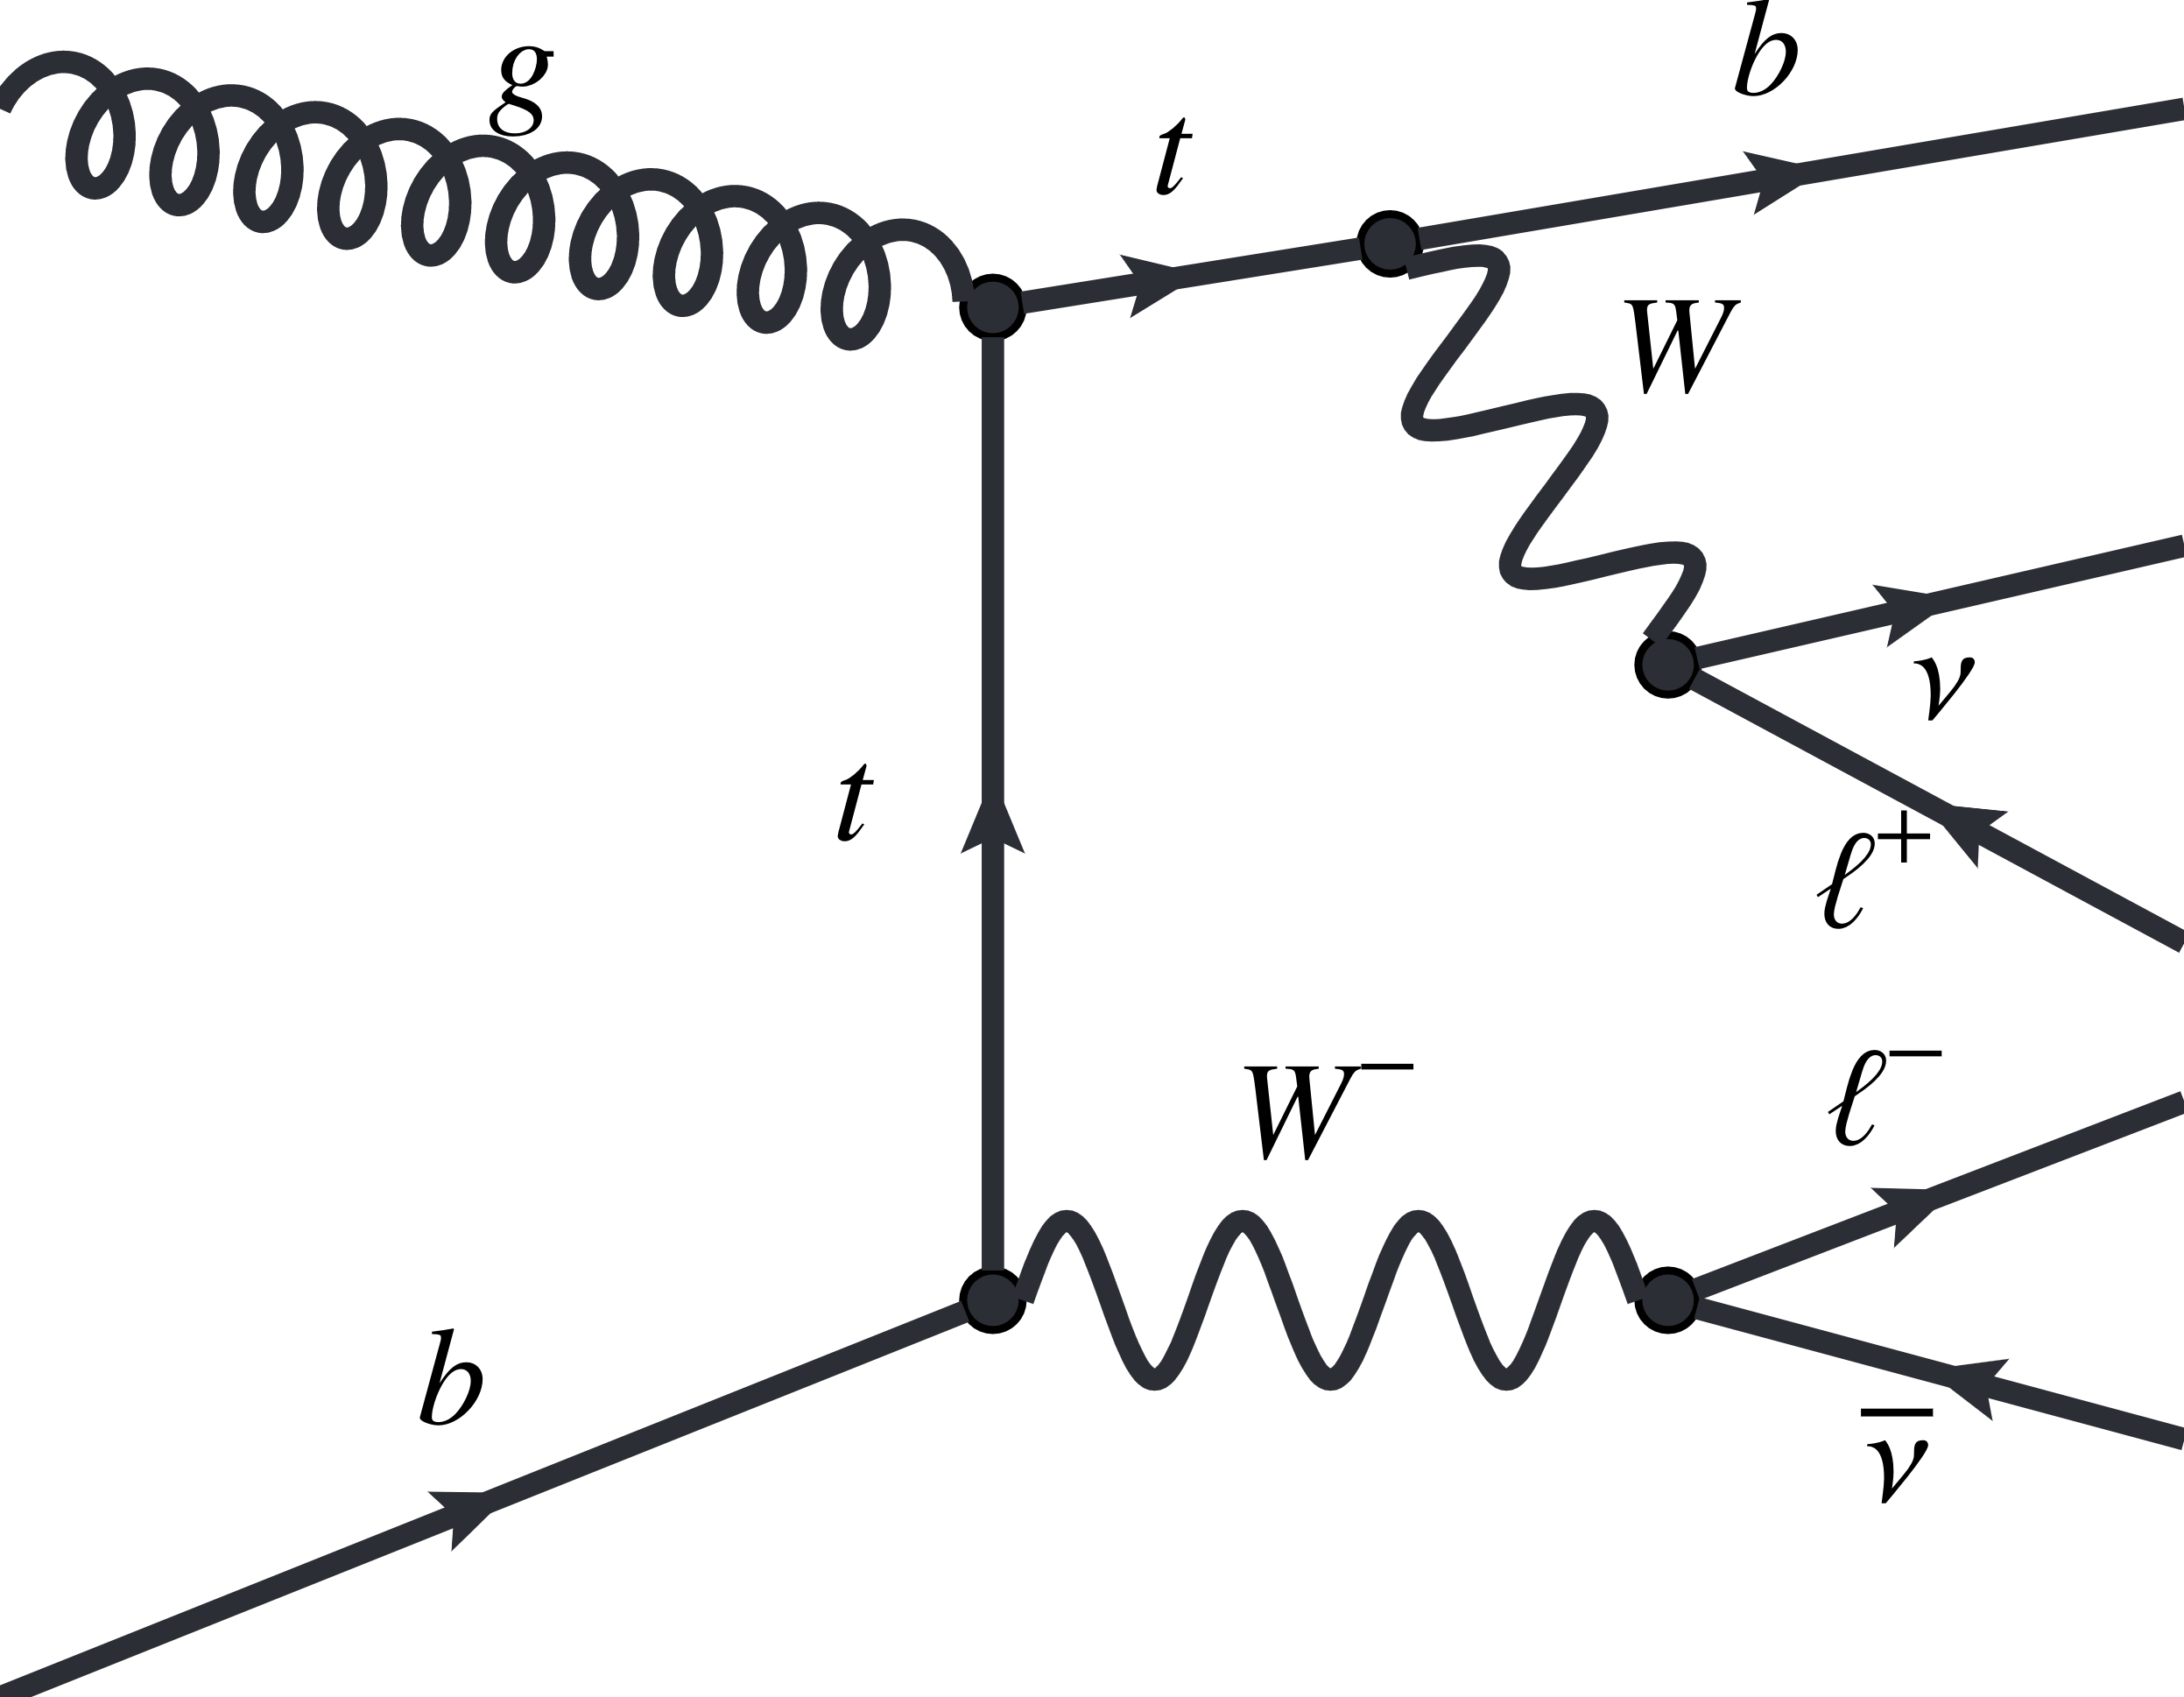
\includegraphics[width = 0.8\textwidth]{tw.png}
        \end{figure}
        \end{column}
        \begin{column}{0.5\textwidth}
        \begin{figure}
            \centering
            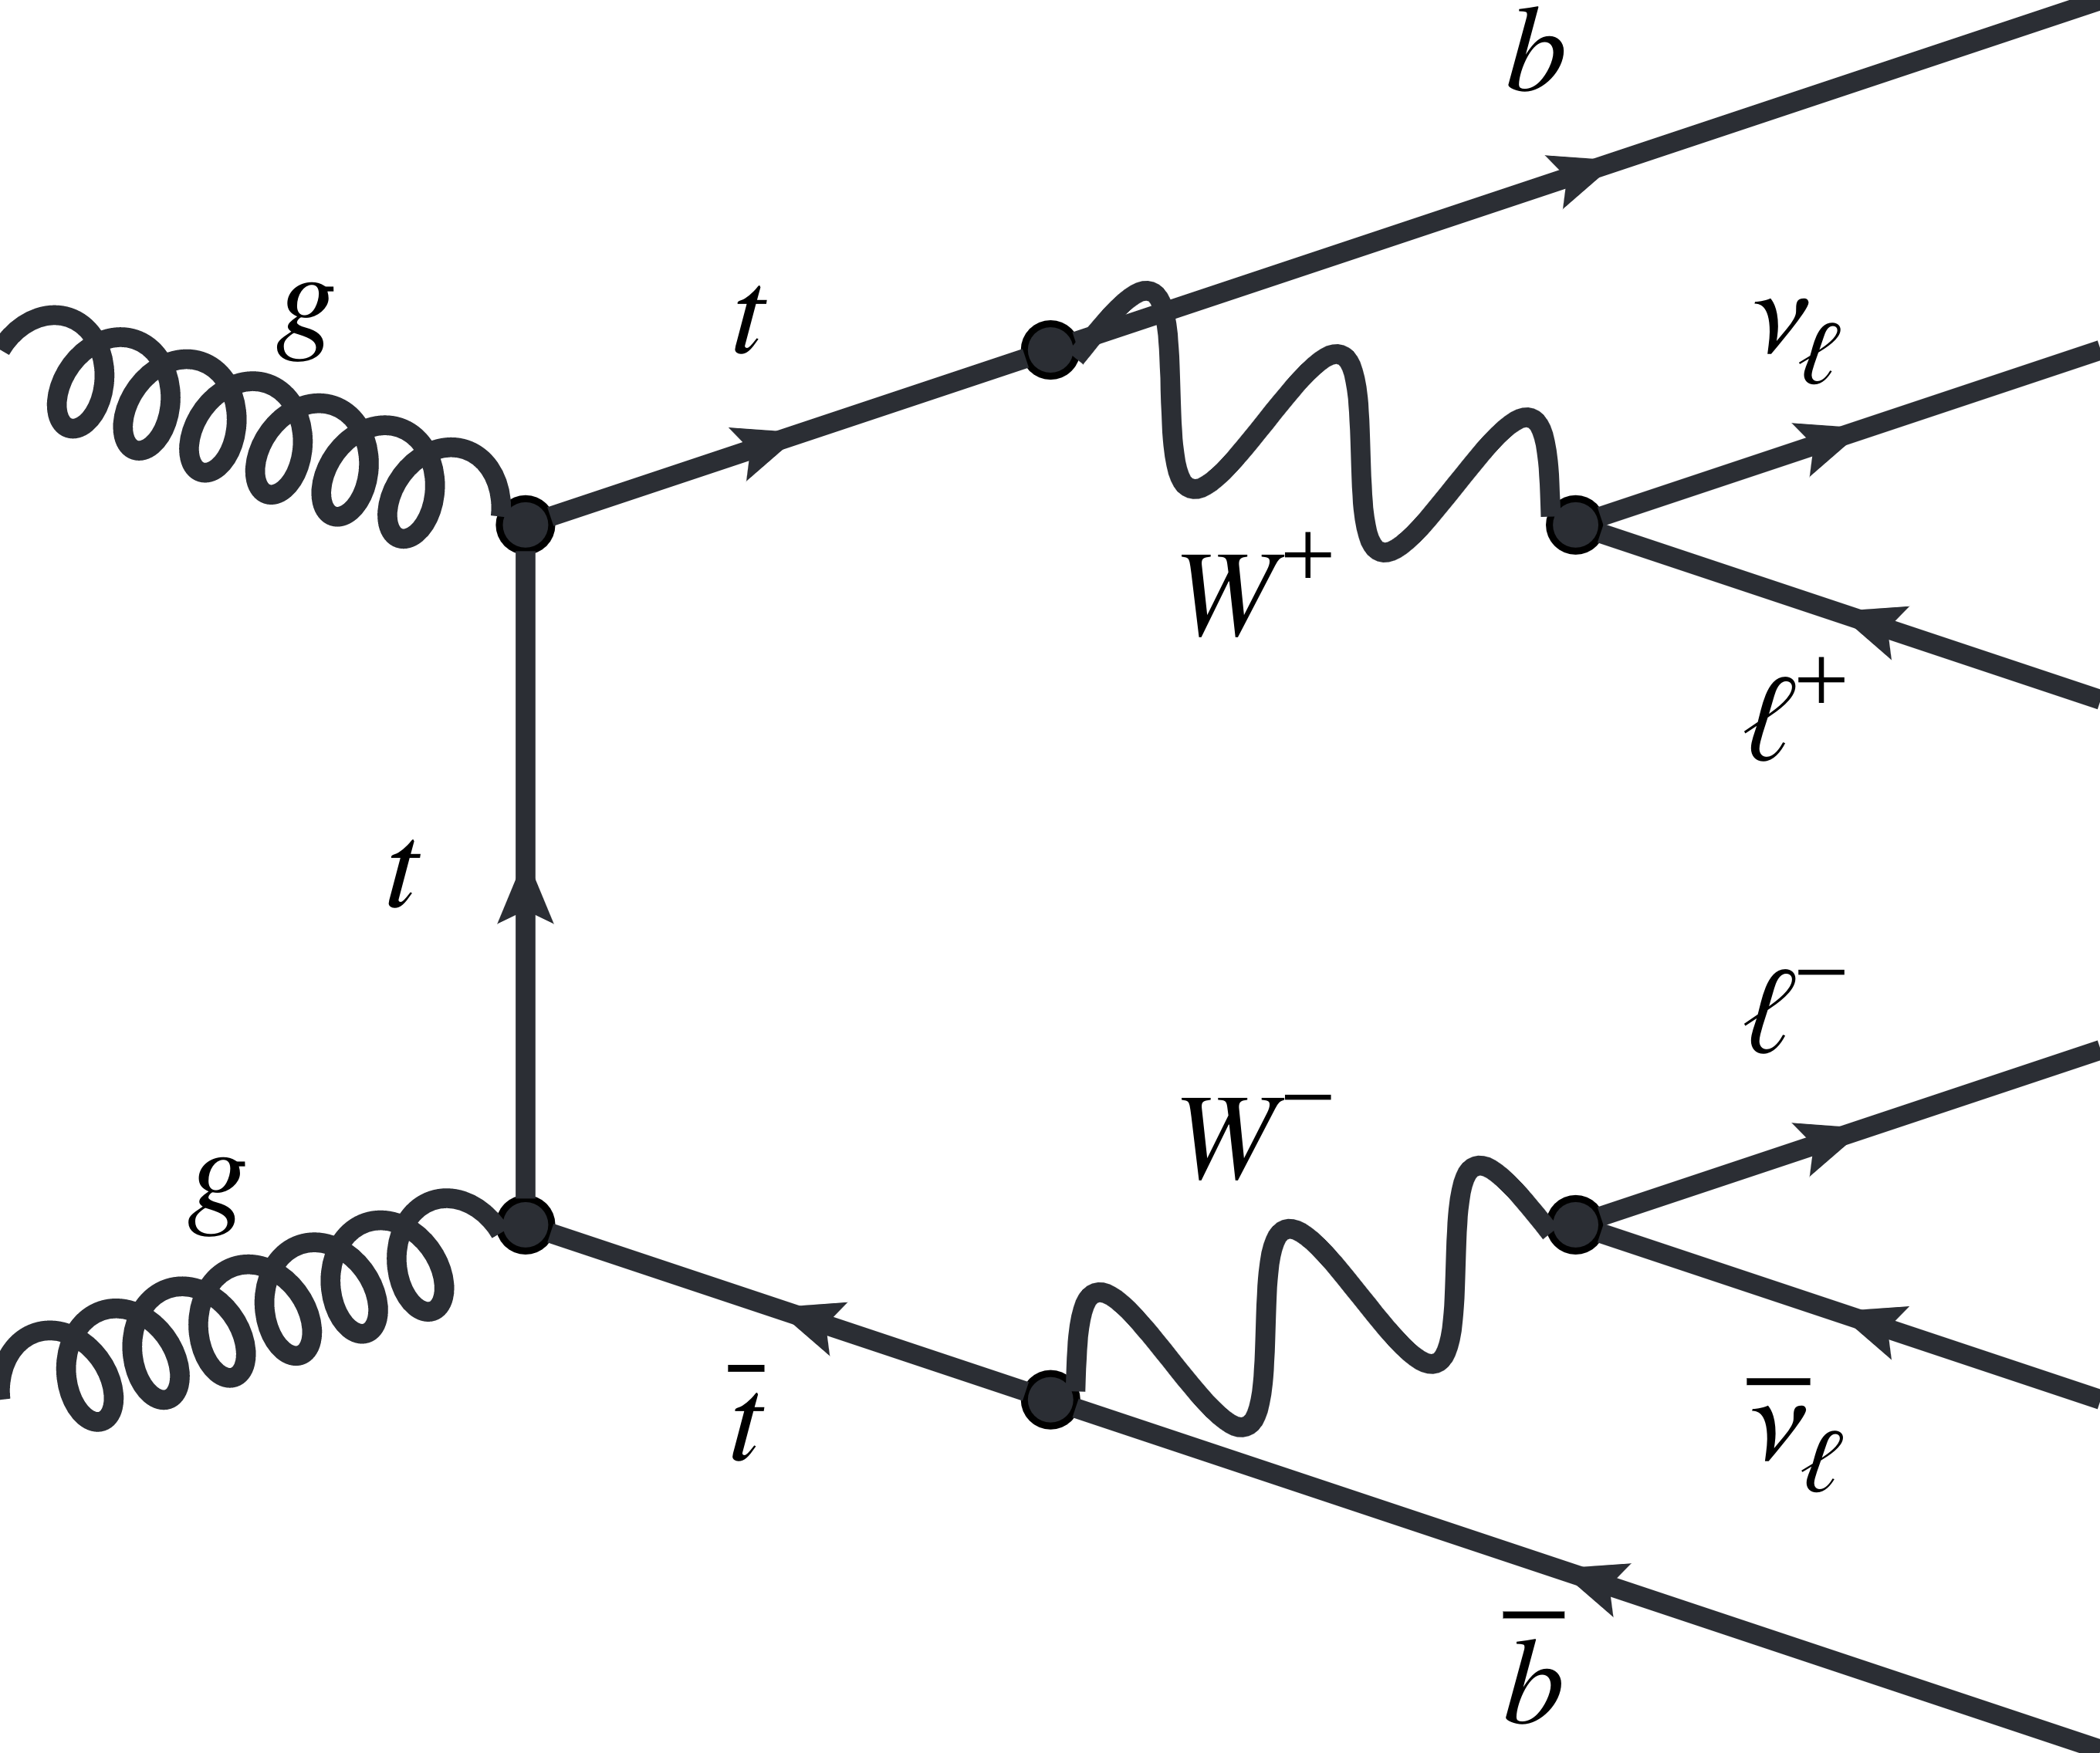
\includegraphics[width = 0.8\textwidth]{tt.png}
        \end{figure}
    \end{column}
\end{columns}
\begin{itemize}
    \item Problem: Cross-sections of $\Ptop\PW$ about 10 times smaller than $\Ptop\APtop$
    \item Interference in NLO order
    \item Instead of applying cut $\longrightarrow$ Neural networks
\end{itemize}
\end{frame}



\begin{frame}{Neural Networks}
\begin{columns}
    \begin{column}{0.5\textwidth}
    \begin{itemize}
        \item Built of layers of simple processors called nodes
        \item Each node is connected to each node in the previous and next layer
        \item Connection: linear function with a weight $\omega$ and a bias $b$ 
        and a non linear activation function $\sigma$
        \item Learning accomplished by backpropagation
    \end{itemize}
    \end{column}
    \begin{column}{0.5\textwidth}
    \begin{figure}
        \centering
        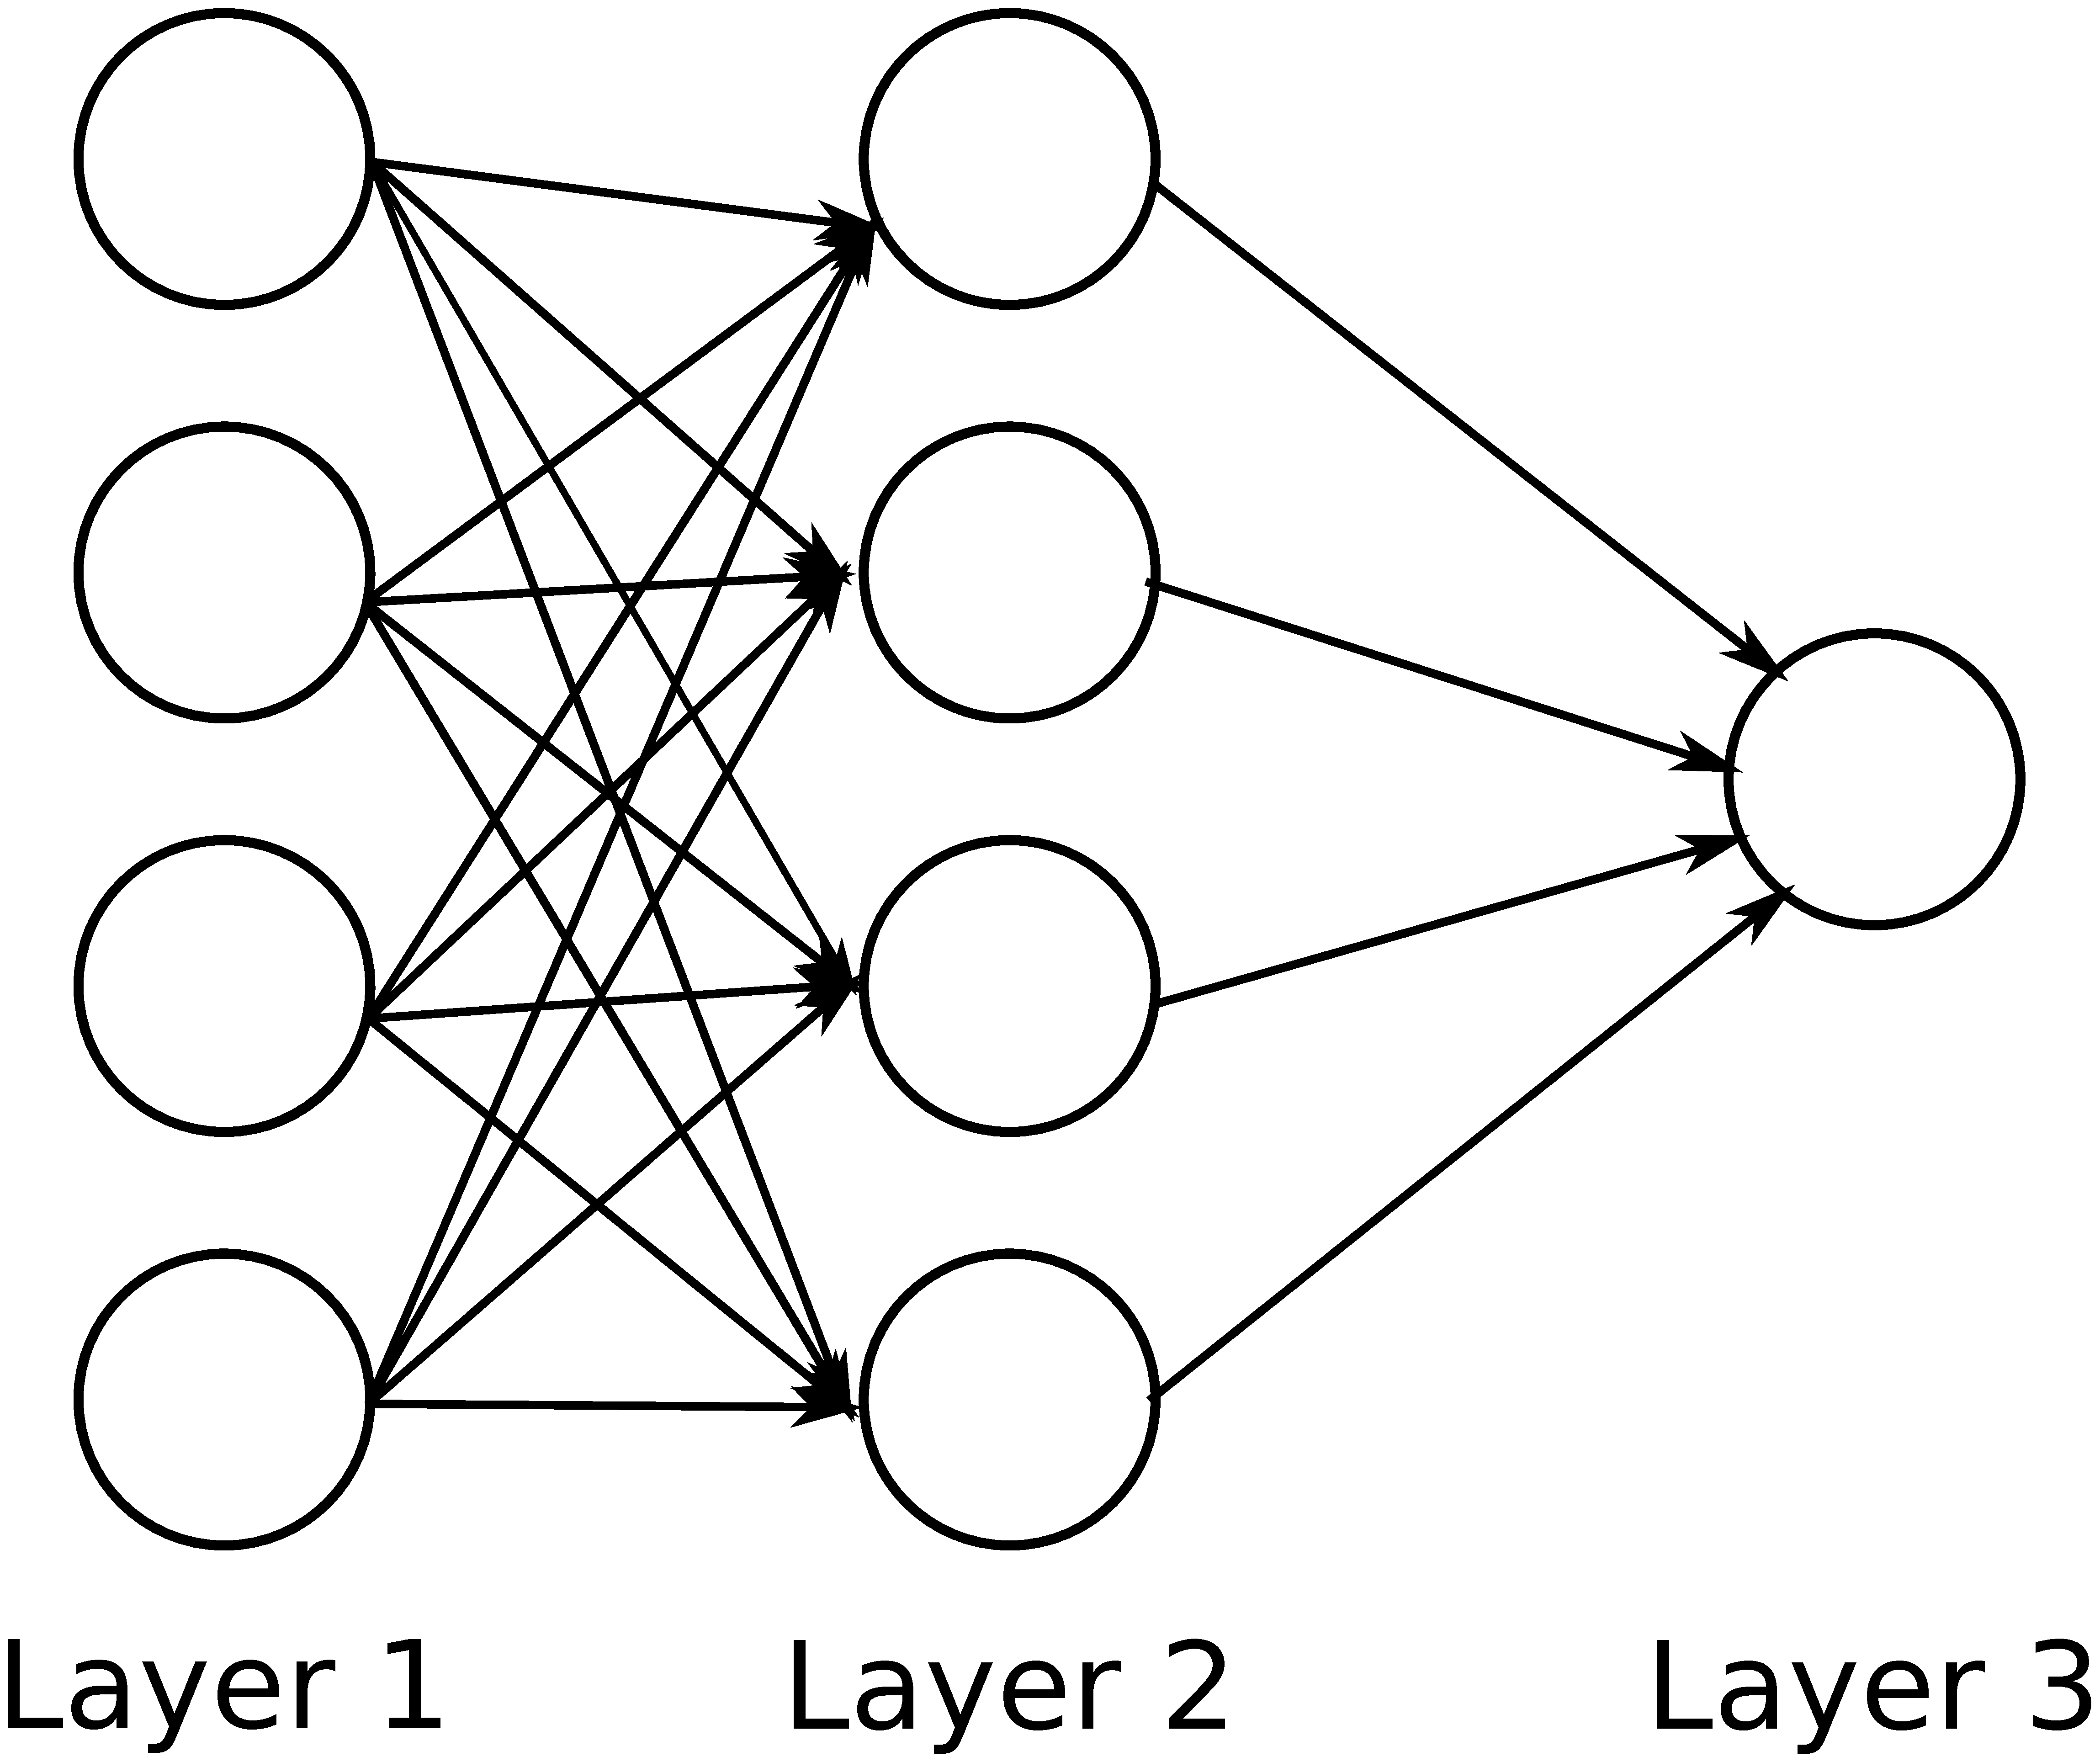
\includegraphics[scale=0.05]{network.eps}
        \label{fig:my_label}
    \end{figure}
    \vspace{0.3cm}
    %\begin{center}
    % $z_j^L = \omega_{jk}^L a_k^{L-1} + b_k$\\
    %    $a_j^L = \sigma ( z_j^L )$
    %\end{center}
    \end{column}
\end{columns}
\end{frame}

\begin{frame}{Loss function and backpropagation}
    \begin{itemize}
        \item Loss = performance estimation, deviation of the model from the truth tag
        \begin{align*}
            \mathcal{L} = -(y \log p + (1 - y) \log (1 - p) )
            \label{eq:binary_crossentropy}
        \end{align*}
        \item Backpropagation estimates the parameters' impact on the cost function using the partial derivatives
        \begin{align*}
            \frac{\partial \mathcal{L}}{\partial a_k^{L-1}} = \sum_{j=1}^N \frac{\partial z_j^L}{\partial a_k^{L-1}} \frac{\partial a_j^L}{\partial z_j^L}\frac{\partial C}{\partial a_j^L}
        \end{align*}
        \item Parameter update following negative gradient
    \end{itemize}
\end{frame}


\begin{frame}{Adversarial Neural Networks}
    \begin{itemize}
        %\item Originally introduced as Generative adversarial %neural networks to overcome weaknesses of generative %networks \cite{2014arXiv1406.2661G}
        \item Neural networks have no info on systematic uncertainties 
        \vspace{0.2cm}
        \item Introduction of a second, adversarial network classifying between nominal and systematic
        \vspace{0.2cm}
        \item Combined loss function $\mathcal{L}_{adversarial}\left( \theta_f, \theta_t \right) = \mathcal{L}(\theta_f) - \mathcal{L}(\theta_f, \theta_r)$
        \vspace{0.2cm}
        \item Network 1: signal/background separation
        \vspace{0.2cm}
        \item Network 2: nominal/systematic separation
        \vspace{0.2cm}
        \item Expectation: network 1 succeeds, network 2 fails
    \end{itemize}
\end{frame}

\begin{frame}{Setup of the ANN}
    \begin{figure}
        \centering
        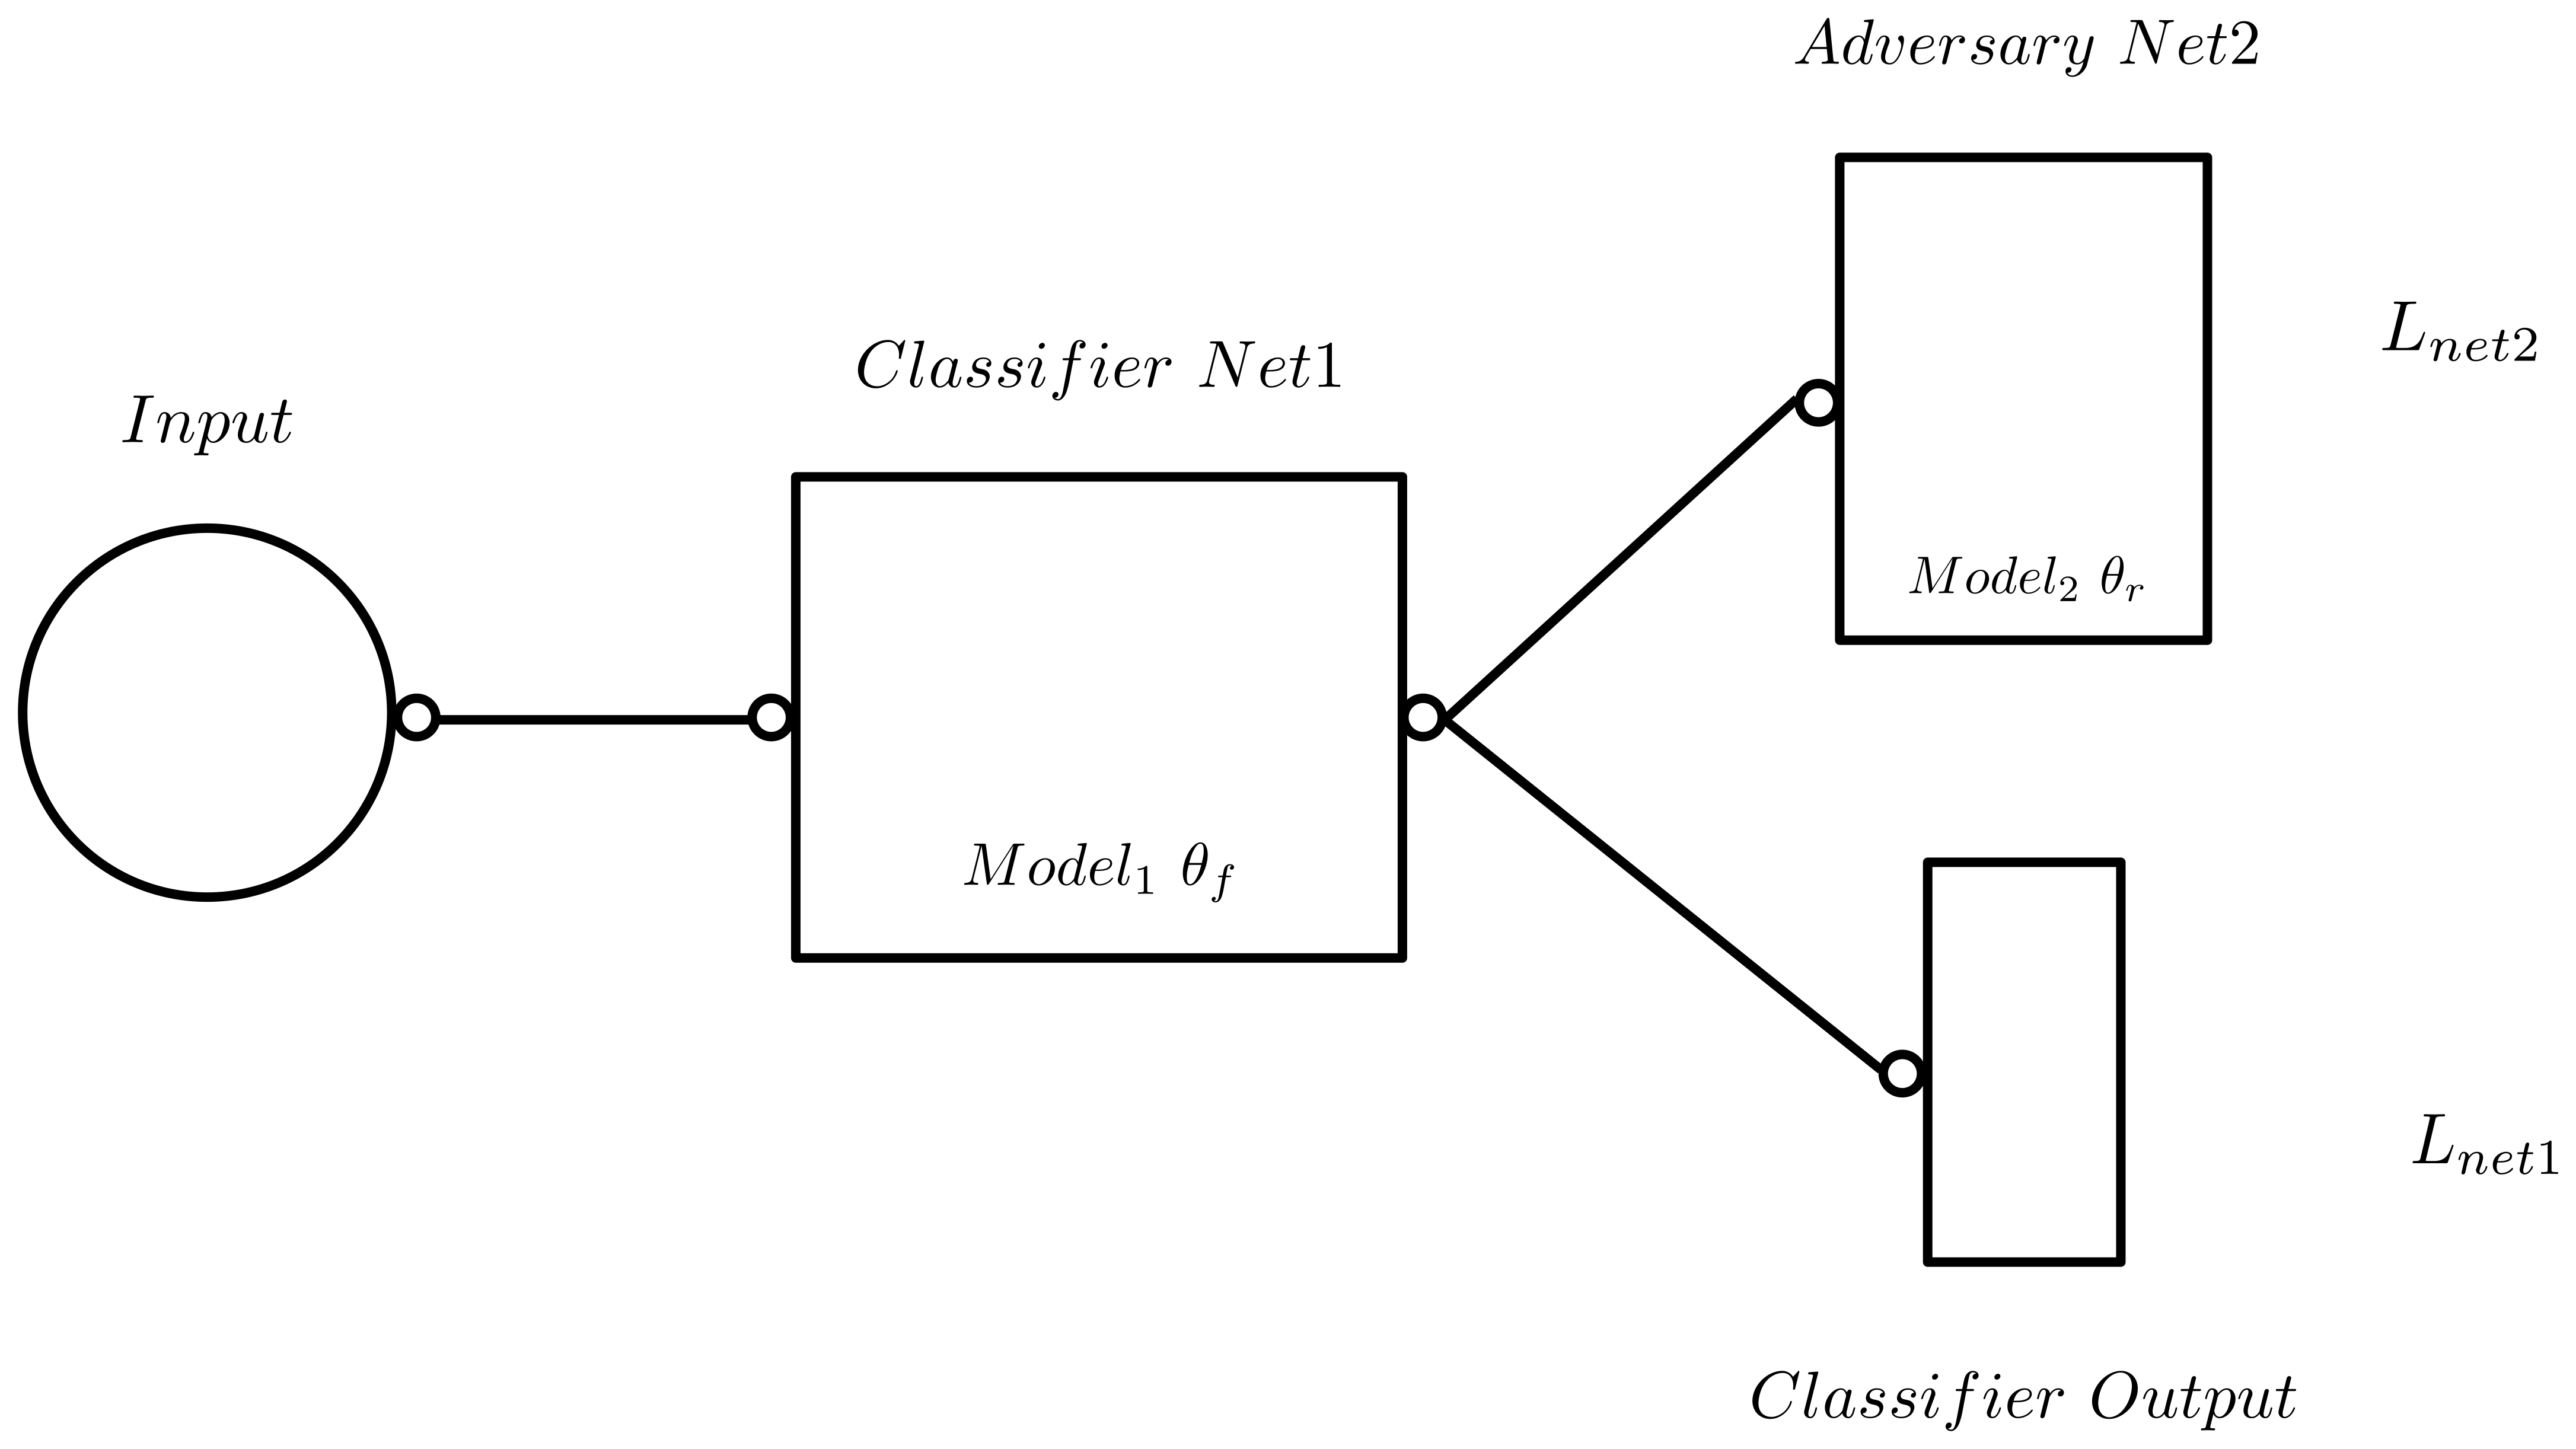
\includegraphics[width=\textwidth]{ANN_sketch.png}
        \label{fig:my_label}
    \end{figure}
\end{frame}

\section{Hyperparameters}



\begin{frame}{Dropout}
\begin{itemize}
    \item Long training and complicated architecture $\rightarrow$ focus on sub-dominant features or mask of the training set
    \item Removes a percentage of nodes for each training step
    \item Disincentives mask of the set or wrong features 
\end{itemize}
\begin{figure}
    \centering
    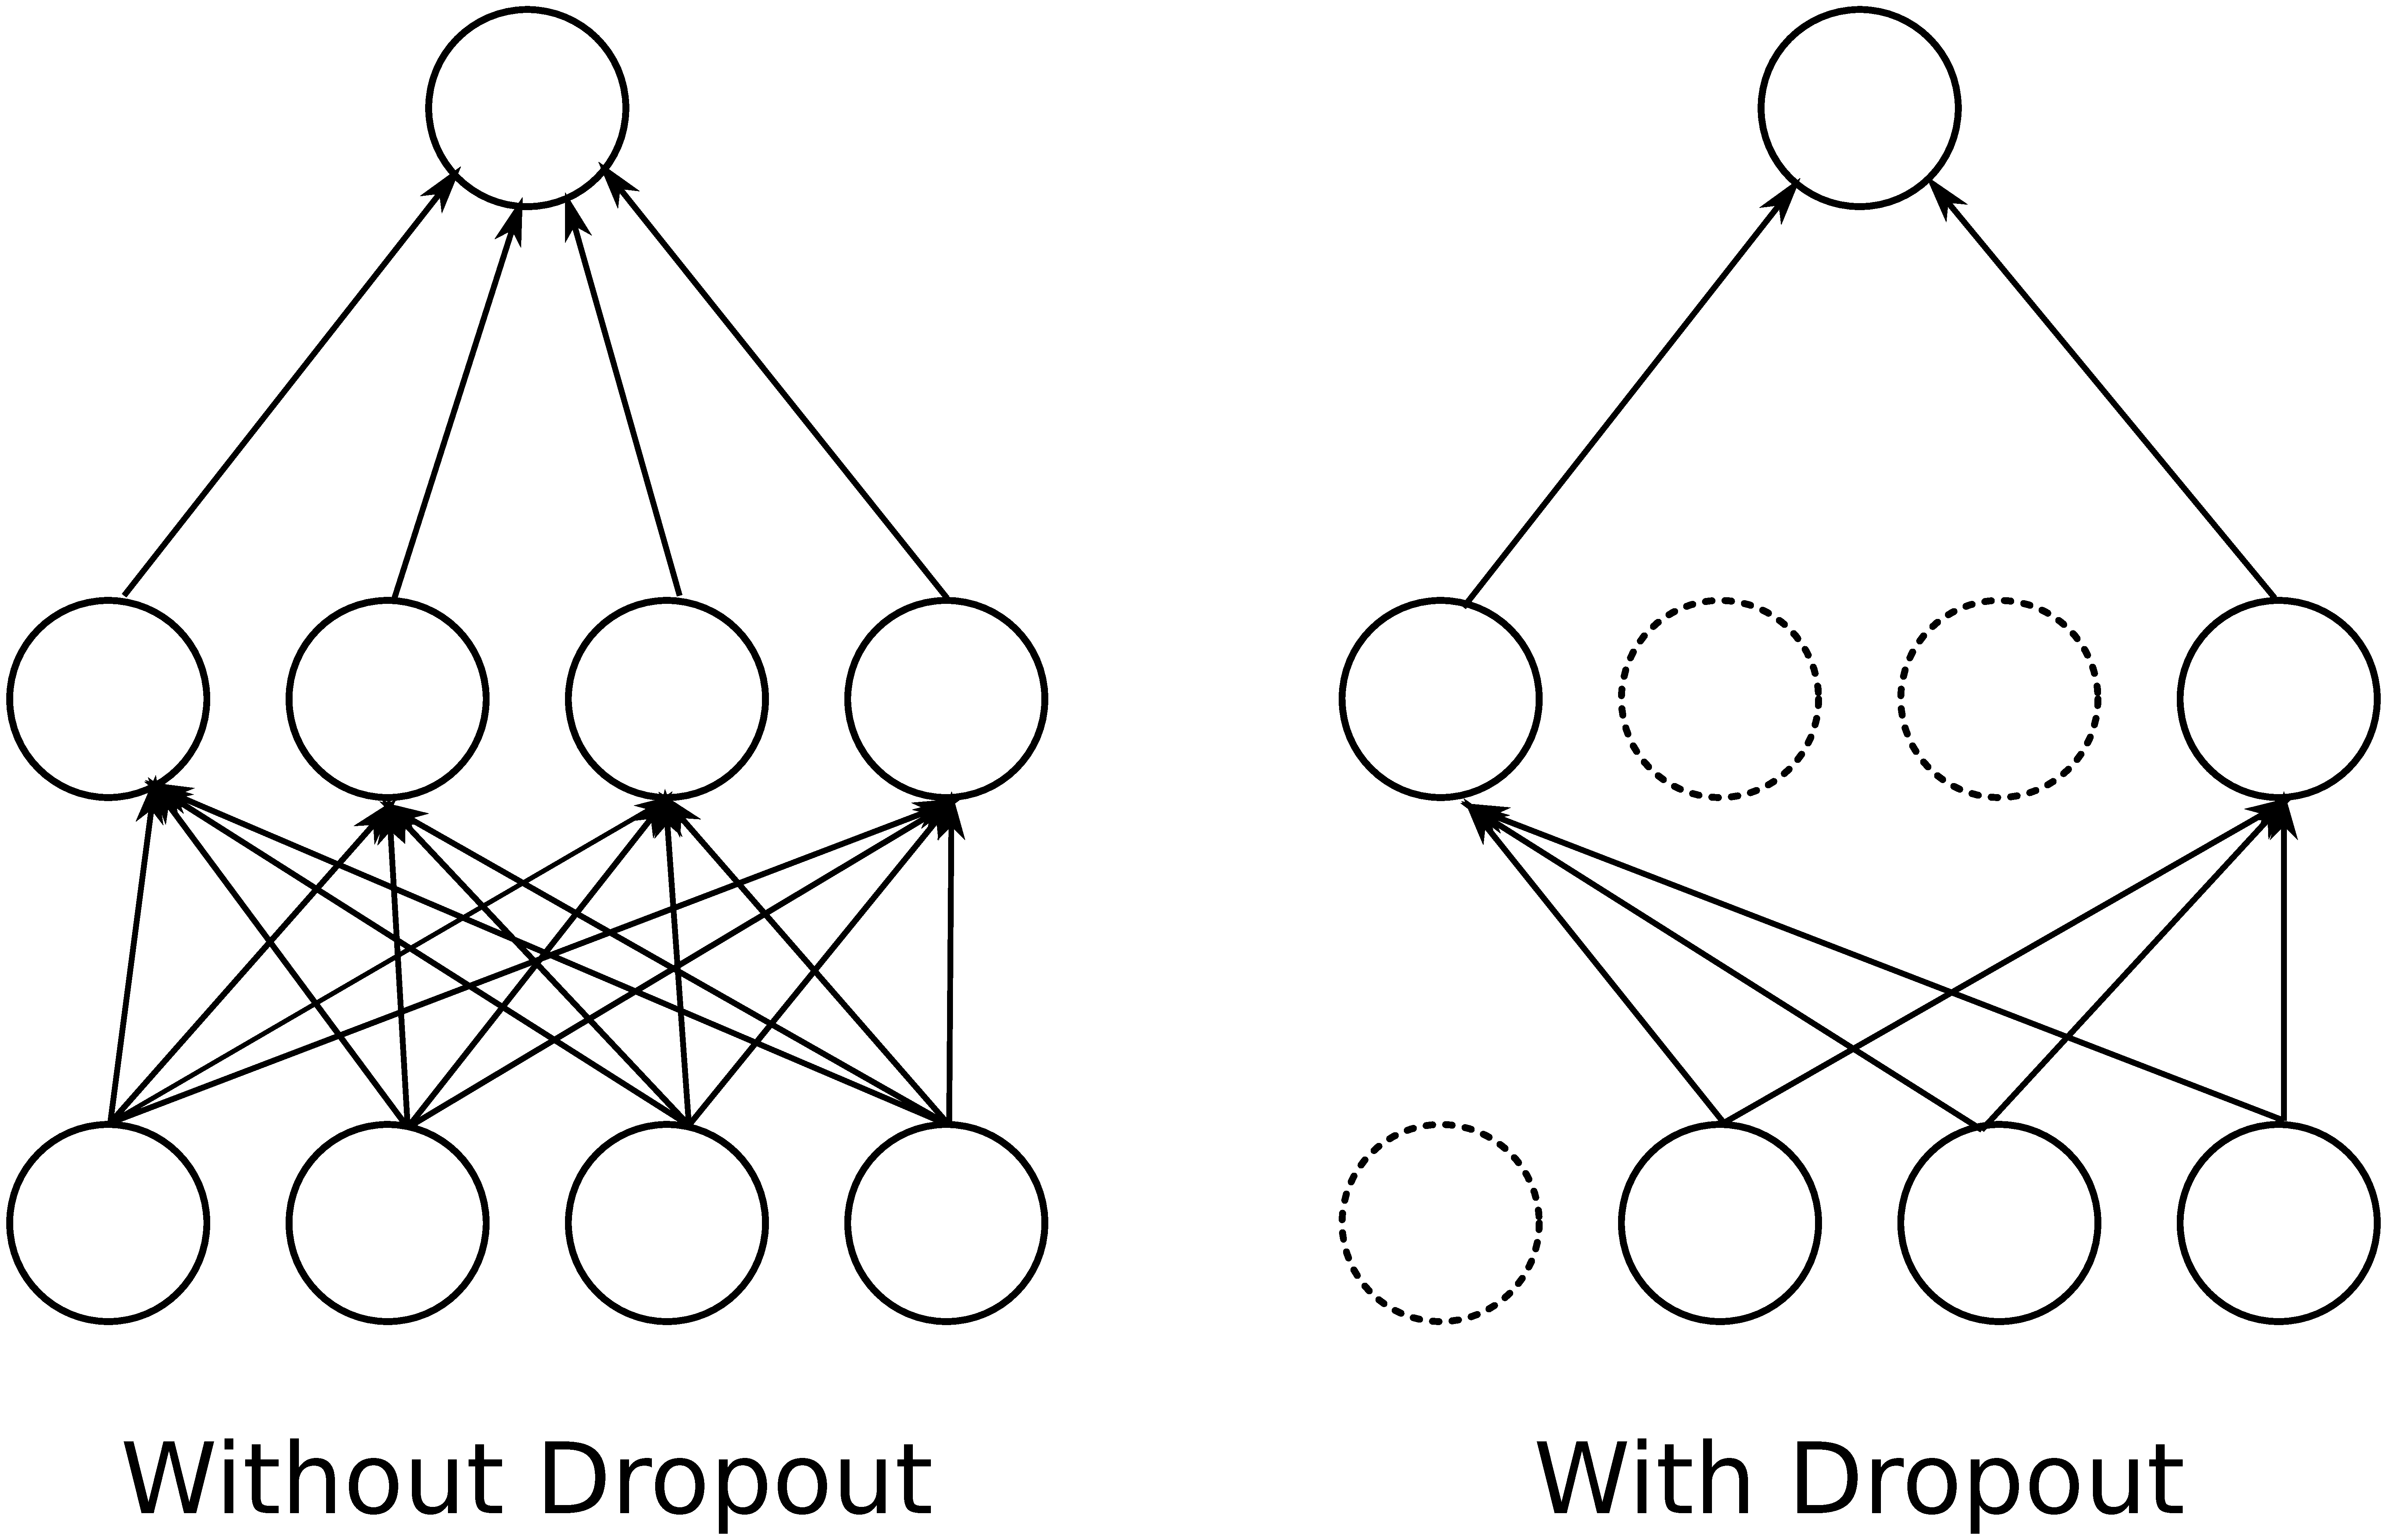
\includegraphics[scale = 0.05]{dropout.eps}
    \label{fig:my_label}
\end{figure}
\end{frame}


\begin{frame}{Impact of dropout on the loss function}
\vspace{-1.2cm}
\begin{column}{0.5\textwidth}
    \begin{figure}
        \centering
        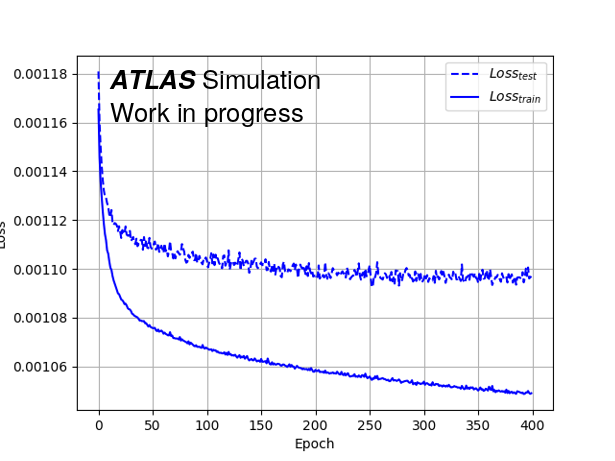
\includegraphics[width=1.1\textwidth]{dropout01.png}
        \caption{Loss curve for dropout = 0.1}
        \label{fig:my_label}
    \end{figure}
\end{column}
\begin{column}{0.5\textwidth}
    \begin{figure}
        \centering
        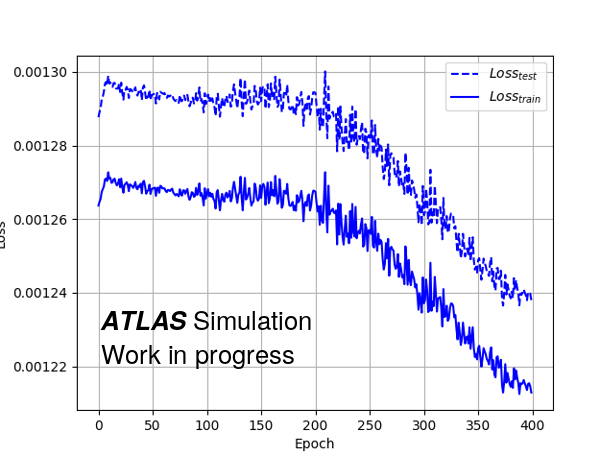
\includegraphics[width=1.1\textwidth]{dropout08.png}
        \caption{Loss curve for dropout = 0.8}
        \label{fig:my_label}
    \end{figure}
\end{column}
\begin{itemize}
    \item For low dropout the training saturates fast
    \item High dropout makes the losses more linear as the training keeps on running
\end{itemize}
\end{frame}

\begin{frame}{Optimisers}
    \begin{itemize}
    \item Gradient based optimisation
        \begin{itemize}
            \item for example SGD, stochastic gradient descent
            \item updates based on negative gradient
            \item Learning rate determines step-size
            \item Step-size does not automatically decay
        \end{itemize}
    \item Adaptive optimisation
        \begin{itemize}
            \item for example Adam, adaptive momentum estimation
            \item learning rate and other parameters get updated based on the past gradients
        \end{itemize}
    \end{itemize}
\end{frame}



\begin{frame}{Results for switching from SGD to Adam}
\vspace{-1cm}
    \begin{column}{0.5\textwidth}
    \begin{figure}
        \centering
        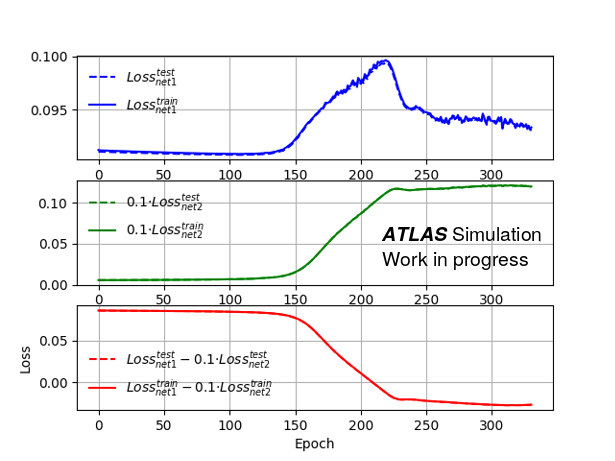
\includegraphics[width=1.1\textwidth]{losses_sgd.png}
        \caption{Loss curve using SGD}
        \label{fig:my_label}
    \end{figure}
\end{column}
\begin{column}{0.5\textwidth}
    \begin{figure}
        \centering
        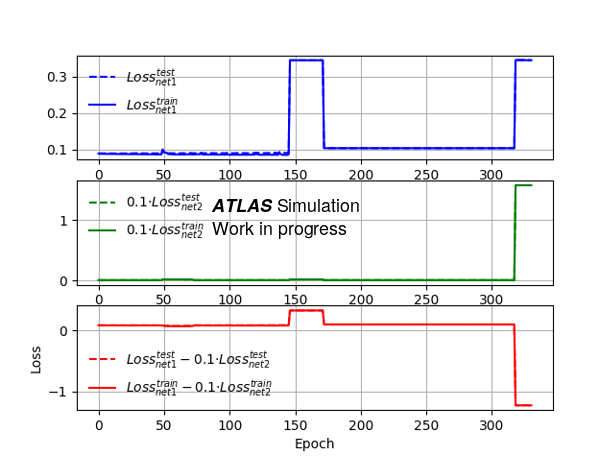
\includegraphics[width=1.1\textwidth]{losses_adam.png}
        \caption{Loss curve using adam}
        \label{fig:my_label}
    \end{figure}
\end{column}
\begin{itemize}
    \item Default optimiser setup is definitely not always a good choice
    \item Also Adam sounds superior to SGD it is not easily interchangeable
\end{itemize}
\end{frame}



\begin{frame}{Learning rate impact}
\vspace{-1.1cm}
    \begin{column}{0.5\textwidth}
    \begin{figure}
        \centering
        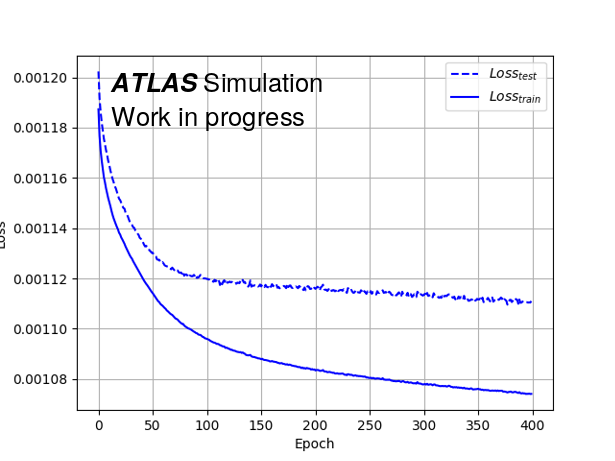
\includegraphics[width=1.1\textwidth]{lr002.png}
        \caption{Using lr = 0.02}
        \label{fig:my_label}
    \end{figure}
\end{column}
\begin{column}{0.5\textwidth}
    \begin{figure}
        \centering
        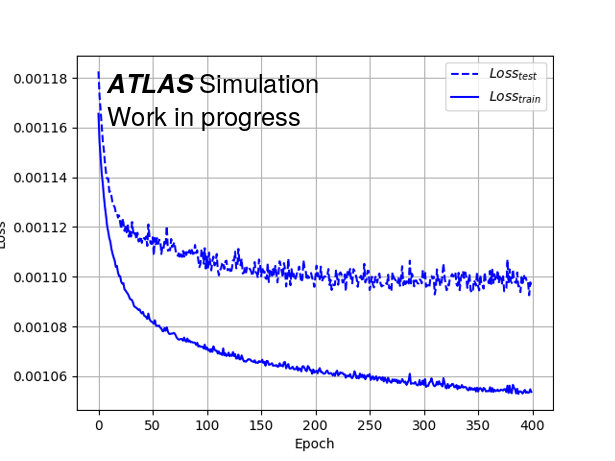
\includegraphics[width=1.1\textwidth]{lr01.png}
        \caption{Using lr = 0.1}
        \label{fig:my_label}
    \end{figure}
\end{column}
\begin{itemize}
    \item High learning rate induces oscillations that might lead to missing a minimum
    \item A low learning rate makes the training converge very slowly
\end{itemize}
\end{frame}

\section{ANN Results}



\begin{frame}{Losses and ROC curve for the adversarial training}
\vspace{-1cm}
    \begin{column}{0.5\textwidth}
    \begin{figure}
        \centering
        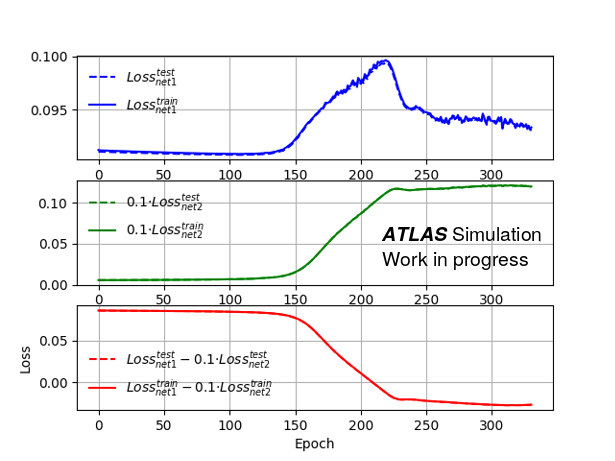
\includegraphics[width=1.1\textwidth]{losses_sgd.png}
        \caption{Loss curves, from top to bottom: Signal/background separation, nominal/systematics separation, combined losses}
        \label{fig:my_label}
    \end{figure}
\end{column}
\begin{column}{0.5\textwidth}
    \begin{figure}
        \centering
        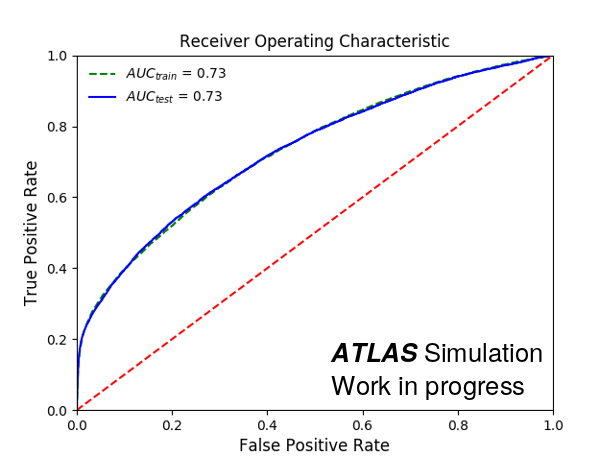
\includegraphics[width=1.1\textwidth]{adver_ROC.png}
        \caption{ROC curve}
        \label{fig:my_label}
    \end{figure}
\end{column}
\begin{itemize}
    \item Maximum for adversary is found
    \item Bad classififer training
\end{itemize}
\end{frame}

\begin{frame}{Separation and Systematics}
\vspace{-1cm}
    \begin{column}{0.5\textwidth}
    \begin{figure}
        \centering
        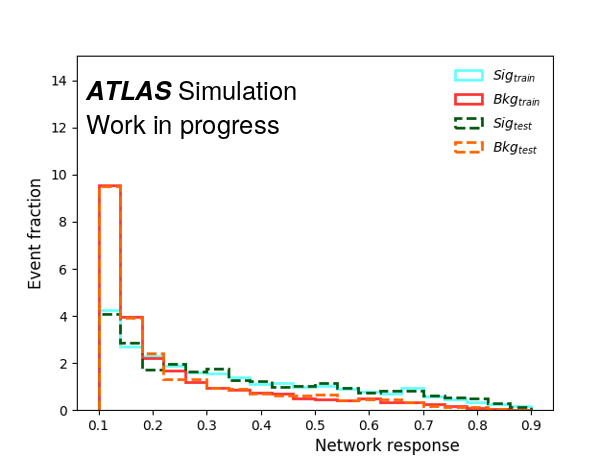
\includegraphics[width=1.1\textwidth]{adver_response.png}
        \caption{Separation}
        \label{fig:my_label}
    \end{figure}
\end{column}
\begin{column}{0.5\textwidth}
    \begin{figure}
        \centering
        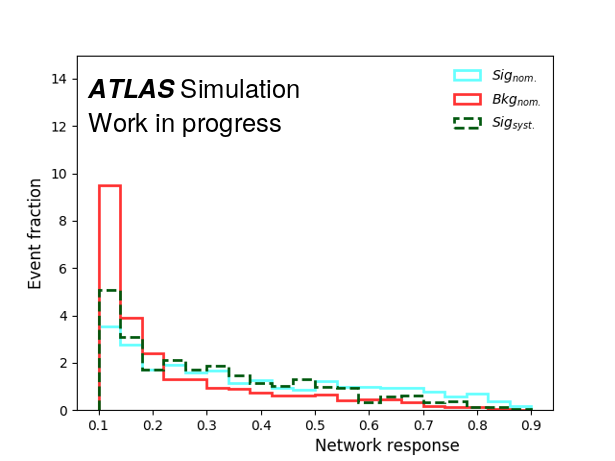
\includegraphics[width=1.1\textwidth]{adver_syst.png}
        \caption{Nominal systematics agreement}
        \label{fig:my_label}
    \end{figure}
\end{column}
\begin{itemize}
    \item The separation is visible. Both networks train.
    \item Neither separation nor nom/sys agreement is very convincing
\end{itemize}
\end{frame}

\begin{frame}{Conclusions}
    \begin{itemize}
        \item Hyperparameters of optimisers and optimisers in general are not always a trivial problem
        \vspace{0.3cm}
        \item The architecture and setup of the network have to be carefully tested and thought out for every problem
        \vspace{0.3cm}
        \item Adversarial neural networks are a promising approach to limit the impact of problematic systematic uncertainties
        \vspace{0.3cm}
        \item In this work the classifier cannot find a model that controls the systematics properly
    \end{itemize}
\end{frame}

%\begin{frame}{Sources}

%\printbibliography
    
%\end{frame}

\end{document}